\RequirePackage{xcolor}
\documentclass{sciposter}
\usepackage{multicol,subfig,amsmath}
\usepackage{graphicx,url,hyperref,doi}
\usepackage[spanish]{babel}   
\usepackage[utf8]{inputenc}
\usepackage[sort&compress,numbers]{natbib}
\usepackage{tikz}
\usepackage{algorithm} 
\usepackage{algpseudocode} 
\usepackage{listings}

\tikzstyle{elem} = [draw, rectangle, thick, minimum height=2em, minimum width=2em]
\tikzstyle{line} = [draw, thick, -stealth, shorten >=1pt]

\setlength{\parskip}{3pt}
\renewcommand{\arraystretch}{1.5}

\title{Nombre de tu proyecto}
\author{Alumno de Verano y Elisa Schaeffer}
\institute {Posgrado en Ingeniería de Sistemas}
\email{alumno.verano@instituto.edu.mx}

\leftlogo[1]{uanl.png} 
\rightlogo[1]{fime.png}

\definecolor{codegreen}{rgb}{0,0.6,0}
\definecolor{codegray}{rgb}{0.5,0.5,0.5}
\definecolor{codepurple}{rgb}{0.58,0,0.82}
\definecolor{backcolour}{rgb}{0.95,0.95,0.92}

\lstdefinestyle{pys}{
    backgroundcolor=\color{white},   
    commentstyle=\color{codegreen},
    keywordstyle=\bfseries\color{blue},
    numberstyle=\tiny\color{codegray},
    stringstyle=\color{codepurple},
    basicstyle=\ttfamily\normalsize,
    breakatwhitespace=false,         
    breaklines=true,                 
    captionpos=b,                    
    keepspaces=true,                 
    numbers=left,                    
    numbersep=25pt,                  
    showspaces=false,                
    showstringspaces=false,
    showtabs=true,                  
    tabsize=2
}
\renewcommand*{\lstlistingname}{Fragmento de código fuente}
\lstset{style=pys}

\begin{document}

\conference{Verano Científico 2021 --- Facultad de Ingeniería Mecánica y Eléctrica --- Universidad Autónoma de Nuevo León}

\maketitle
\begin{abstract}
En el resumen describes brevemente todo el proyecto, desde qué se trata hasta qué lograste hacer.
\end{abstract}

\begin{multicols}{2} 

\section{Introducción}

De qué se trata el proyecto. Hipótesis y objetivos. Motivación, justificación.

\section{Antecedentes}

Conceptos y notación indispensables para que tus lectores puedan entender el resto del trabajo. Citamos al libros de texto como el de \citet{ai}.

\section{Estado de arte}

Qué han hecho los demás sobre este tema (citar a publicaciones científicas, de preferencia publicadas en revistas que tengan DOI y que por lo menos algunos sean de los últimos cinco años. Aquí se suelen citar artículos como por ejemplo el trabajo de \citet{elisa} o algo que se haya presentado en un congreso como \citet{ar}. A veces es necesario definir algo matemático como por ejemplo
\begin{equation}
    f(x) = \sum_{i = 0}^\infty \sin(i x)
    \label{suma}
\end{equation}
para comunicar mejor lo que pasa. Si una ecuación depende de otra, conviene mencionarlo de manera explícita.
Por ejemplo en $g(x) = \sqrt{f(x)}$, $f(x)$ proviene de la ecuación \eqref{suma}.

Área de oportunidad: qué exactamente este trabajo contribuirá encima de lo que ya existe.  {\textquestiondown}Qué tiene de diferente/original/impacto?

\section{Solución propuesta}

Metodología, herramientas (qué en sí haces, cómo lo haces, con qué lo haces).
La implementación se hizo en Python 3.9 \citep{python} y los componentes se interconectan como muestra el diagrama de la figura \ref{diag}.

\begin{figure}
\captionsetup{type=figure} % por culpa de sciposter
\setcounter{figure}{0} % por culpa de sciposter
\begin{center}
    \begin{tikzpicture}[]
      \matrix[row sep=0.5cm]{
      \node[elem] (n1) {Una cosa}; & & \node[elem] (n2) {Otra cosa}; \\
      & \node[elem] (n3) {Nueva cosa}; & \\
      };
     \draw [line] (n1) -- (n2);
     \draw [line] (n1) -- (n3);
     \draw [line] (n2) -- (n3);
    \end{tikzpicture}
\end{center}
\caption{Hay que explicar qué quieren decir los elementos de la figura.}
\label{diag}
\end{figure}

Los pasos del procecimiento propuesto se pueden expresar con un {\em pseudocódigo}:

\begin{algorithmic}[1]
\State $x \leftarrow 0$
\For {$i \in [1,2,\ldots, n]$}
	\State $x \leftarrow x + i$
\EndFor
\If {$x < \beta$}
    \State $d \leftarrow \top$
\EndIf
\end{algorithmic} 

Otra posibilidad es incluir algo de código tal cual:
\begin{lstlisting}[language=Python, caption=Procedimiento del segundo paso]
import numpy as np
from numpy.random import uniform
X = uniform(size = (3, 5))
print(np.shape(X))
\end{lstlisting}

\section{Experimentos}

Diseño, reportaje y análisis de los resultados de los experimentos. Por lo general se incluyen figuras como la figura \ref{curvas}.

\begin{figure}
\setcounter{figure}{1} % por culpa de sciposter
\captionsetup{type=figure} % por culpa de sciposter
\begin{center}
   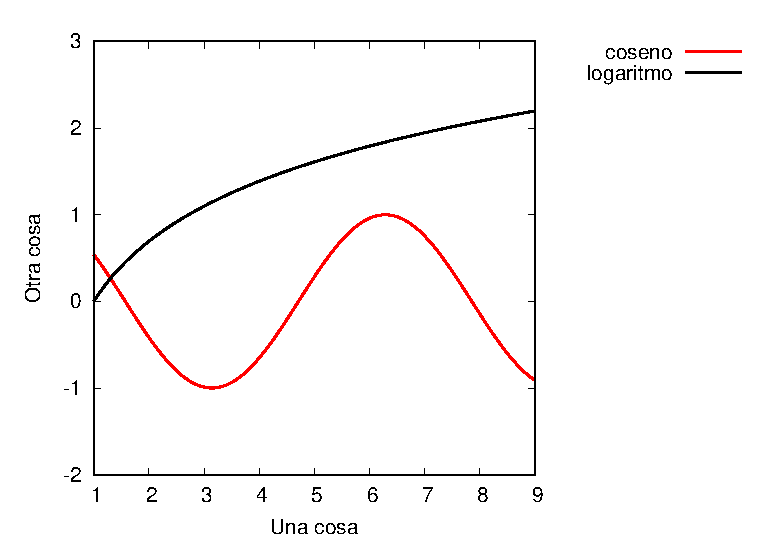
\includegraphics[width=0.5\textwidth]{curvas.eps}
   \end{center}
    \caption{Hay que explicar qué quieren decir los elementos de la figura.}
    \label{curvas}
\end{figure}

Además es muy común incluir cuadros de datos, como por ejemplo el cuadro \ref{data}.

\begin{table}
\setcounter{table}{0} % por culpa de sciposter
\captionsetup{type=table} % por culpa de sciposter
\caption{Aquí explicas cómo interpreta el cuadro.}
\label{data}
\begin{center}
\scalebox{0.9}{\begin{tabular}{|r|c|l|}
    \hline
         \multicolumn{1}{|c|}{\rotatebox{90}{\bf Valor}}
         & \multicolumn{1}{|c|}{\rotatebox{90}{\bf Parámetro}}
         & \multicolumn{1}{|c|}{\rotatebox{90}{\bf Descripción\phantom{m}}} \\
         \hline
         0.23 & $x$ & algo \\
         \hline
         2.34 & $y$ & demo \\
        \hline
    \end{tabular}}
\end{center}
\end{table}

\section{Conclusiones}

Qué se logró hacer; qué posibilidad de trabajo a futuro se tiene para este trabajo.

\subsection*{Agradecimientos}

Organismos que otorgaron beca. Las demás personas que no son autores que ayudaron en algo. El póster se preparó con \url{https://www.overleaf.com/}.

\end{multicols}

\bibliography{poster}
\bibliographystyle{plainnat}

\end{document}